\documentclass[10pt, aspectratio=169]{beamer}

% --- Pacchetti Standard ---
\usepackage[utf8]{inputenc}
\usepackage[italian]{babel}
\usepackage{amsmath}
\usepackage{amsfonts}
\usepackage{amssymb}
\usepackage{graphicx}
\usepackage{booktabs}
\usepackage{tikz}
\usepackage[most]{tcolorbox}
% --- Tema e Colori ---
\usetheme{Madrid}
\usecolortheme{default}
\setbeamertemplate{navigation symbols}{}

\definecolor{myblue}{RGB}{0, 76, 153}
\setbeamercolor{title}{fg=white, bg=myblue}
\setbeamercolor{frametitle}{fg=white, bg=myblue}

\title[P.A.S.H.]{Sviluppo di Protesi di Piede Passive ad Alto Cushioning}
\author{Andrea Diano, Andrea Goriani, Riccardo Mambrini}
\date{\today}
% Nel preambolo — richiede \usepackage{tikz}

\begin{document}
% ============================================================
% SLIDE TITOLO — loghi centrati in alto
% ============================================================
\begin{frame}[plain]

    % ── Riga loghi ──────────────────────────────────────────
    \begin{center}
      
\includegraphics[height=2.4cm, keepaspectratio]{image/logo_santanna.png}
      \hspace{1.2cm}
      \includegraphics[height=2.4cm, keepaspectratio]{image/felixstride_logo.png}
    \end{center}

    \vspace{0.2cm}
    {\color{myblue}\rule{\linewidth}{1.5pt}}
    \vspace{0.2cm}

    \begin{center}
      {\color{myblue}\Large\bfseries P.A.S.H. - Parallel Adaptive Stiffness Heel}\\[0.55cm]
      {\small Andrea Diano \quad $\cdot$ \quad Andrea Goriani \quad $\cdot$ \quad Riccardo Mambrini}\\[0.15cm]
      {\footnotesize\itshape Istituto di BioRobotica — Scuola Superiore Sant'Anna, Pisa}\\[0.15cm]
      {\footnotesize \today}
    \end{center}

    \vspace{0.2cm}
    {\color{myblue}\rule{\linewidth}{1pt}}

\end{frame}
%% ============================================================
% SLIDE TITOLO — logo centrato in alto
% ============================================================
\begin{frame}[plain]

    \begin{center}
      % Logo centrato in alto
      
\includegraphics[width=0.45\textwidth]{image/logo_santanna.png}
    \end{center}

    \vspace{0.2cm}
    {\color{myblue}\rule{\linewidth}{1.5pt}}
    \vspace{0.2cm}

    \begin{center}
      {\color{myblue}\Large\bfseries P.A.S.H. - Parallel Adaptive Stiffness Heel}\\[0.55cm]
      {\small Andrea Diano \quad $\cdot$ \quad Andrea Goriani \quad $\cdot$ \quad Riccardo Mambrini}\\[0.15cm]
      {\footnotesize\itshape Istituto di BioRobotica — Scuola Superiore Sant'Anna, Pisa}\\[0.15cm]
      {\footnotesize \today}
    \end{center}

    \vspace{0.2cm}
    {\color{myblue}\rule{\linewidth}{1pt}}

\end{frame}
% --- PREAMBOLO: definisci i colori dei blocchi ---
\definecolor{colorWalking}{RGB}{213, 229, 242}    % azzurro — Daily Walking
\definecolor{colorRunning}{RGB}{249, 224, 210}    % pesca   — Sport & Running
\definecolor{colorTerrain}{RGB}{220, 235, 215}    % verde   — Uneven Terrain
\definecolor{colorAccess} {RGB}{224, 218, 238}    % lavanda — Global Accessibility
\definecolor{blockText}   {RGB}{40,  40,  40}     % testo scuro uniforme

% --- SLIDE 1: PROBLEM IDENTIFICATION & CONTEXT ---
\begin{frame}{Problem Identification \& Context: The Limits of Passive Prostheses}
    \begin{columns}[T]
        \begin{column}{0.45\textwidth}
            \vspace{0.5cm}
            \begin{figure}
                \centering
                \begin{figure}
                    \centering
                    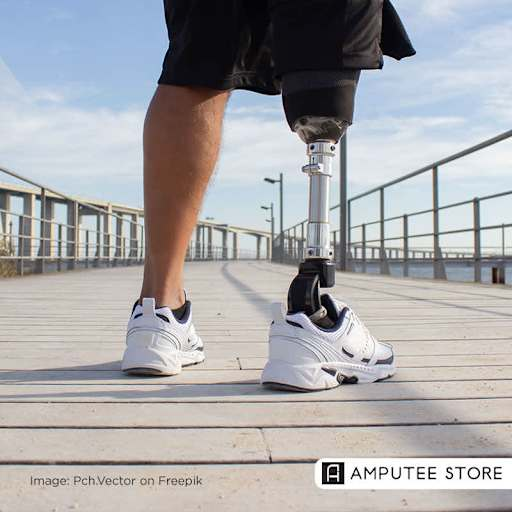
\includegraphics[width=\textwidth, height=3.5cm, keepaspectratio]{image/slide_1.jpg}
                    \caption{{Transtibial amputee with passive prosthesis}}
                \end{figure}
            \end{figure}
        \end{column}
        \begin{column}{0.55\textwidth}
            \vspace{-0.75em}
            \begin{itemize}
                \item \textbf{Context:}
                \begin{itemize} 
                    \item Passive prostheses dominate the market for their reliability and low cost.
                    \item They exhibit a \alert{fixed dynamic response}.
                \end{itemize}
                \item \textbf{Biomechanical Problem:}
                \begin{itemize}
                    \item \textit{Task-invariant response:} fixed stiffness cannot adapt between walking, running, or stair climbing.
                    \item \textit{Terrain-blind mechanics:} no impedance modulation.
                \end{itemize}
                \item \textbf{The Dilemma (Deformability vs. Energy):}
                \begin{itemize}
                    \item \textit{Soft} heel: absorbs impact but dissipates energy.
                    \item \textit{Rigid} heel: returns energy but damages the residual limb.
                \end{itemize}
                \item \textbf{Project Goals:}
                \begin{itemize}
                    \item \textbf{Zero Electronics:} No batteries, no sensors.
                    \item \textbf{Low-Maintenance:} High durability and low cost.
                    \item \textbf{Dynamic Cushioning:} Impact response optimization.
                \end{itemize}
            \end{itemize}
        \end{column}
    \end{columns}
\end{frame} % Ric

% --- SLIDE 2: BIOMECHANICS ---
\begin{frame}{Biomechanics of Locomotion and Gait Dynamics}
    \begin{columns}[T]
        \begin{column}{0.45\textwidth}
            \begin{figure}
                \centering
                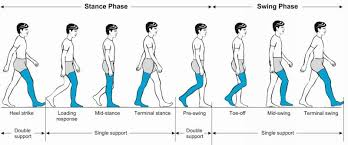
\includegraphics[width=\linewidth]{image/gait.jpeg}
                \caption{ Gait Cycle diagram (60\% Stance / 40\% Swing)}
            \end{figure}
            \vspace{-1.5em}
            \begin{block}{Froude Number ($Fr$)}
                \[ Fr = \frac{v^2}{g \cdot L} \]
                \centering \small Critical threshold $\approx 0.5$ for the walk-to-run transition.
            \end{block}
        \end{column}
        \begin{column}{0.55\textwidth}
            \begin{itemize}
                \item \textbf{Gait Cycle:} 
                \begin{itemize}
                    \item Transition between \textit{Stance Phase} (load absorption/push-off)
                    \item \textit{Swing Phase} (pendulum effect).
                \end{itemize}
                \item \textbf{Speed Parameters:} 
                \begin{itemize} 
                    \item Governed by \textit{Stride Length} 
                    \item \textit{Step Frequency}. Increasing frequency distributes the load over time. 
                \end{itemize}
                \item \textbf{Focus: Heel Strike \& Roll-over:}
                \begin{itemize}
                    \item Heel contact is the point of maximum stress at the \alert{residual limb–socket interface}.
                    \item Smooth roll-over is essential to minimize metabolic cost.
                \end{itemize}
                \item \textbf{Strategic Choice:} 
                \begin{itemize}
                    \item Cushioning localized at the heel. 
                    \item The forefoot remains rigid to ensure push-off (\textit{Toe-off}).
                \end{itemize}
            \end{itemize}
        \end{column}
    \end{columns}
\end{frame} % Ric

% --- SLIDE 3: STATE OF THE ART ---
\begin{frame}{State of the Art: Passive Prosthetic Feet Overview}
    \begin{columns}[T]
        \begin{column}{\textwidth}
            \centering
            \vspace{-2em}
            % Tre immagini affiancate — sostituisci i nomi file con le tue foto
            \begin{figure}
                \centering
                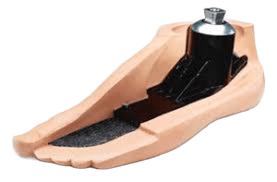
\includegraphics[width=0.21\linewidth]{image/sach.png}
                \hspace{3em}%\hfill
                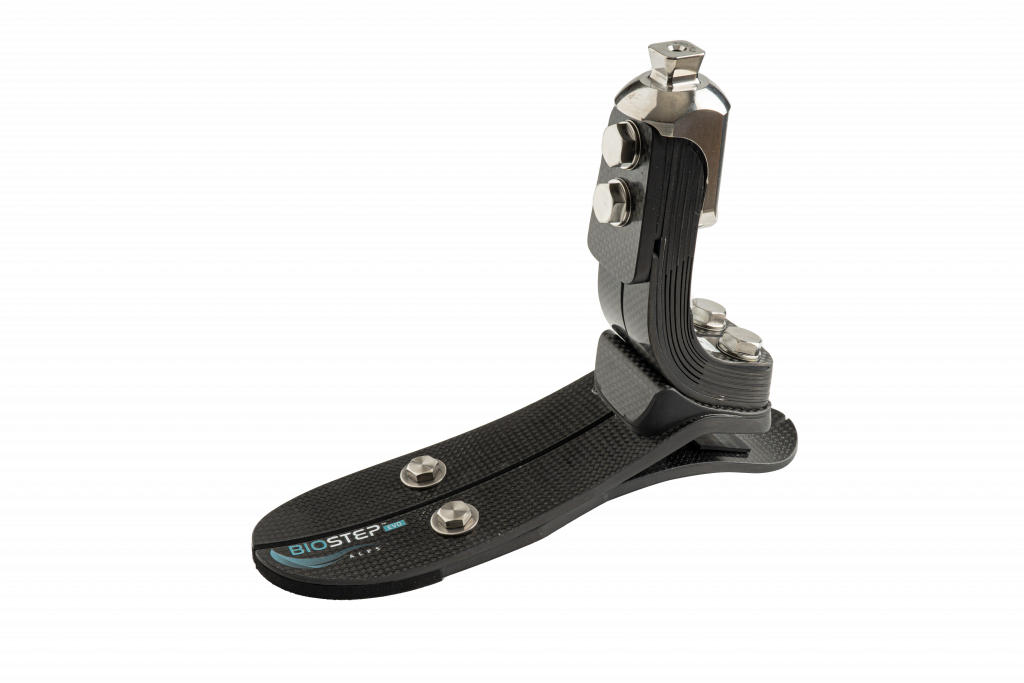
\includegraphics[width=0.21\linewidth]{image/esr_prostesis.png}
                \hspace{3em}%\hfill
                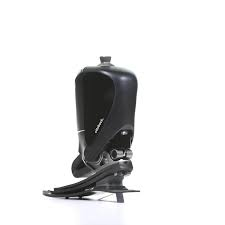
\includegraphics[width=0.21\linewidth]{image/ottobock.jpeg}
            \end{figure}

            \vspace{0.2cm}

            \begin{tabular}{p{4.5cm} p{4.5cm} p{4.5cm}}
                \toprule
                \textbf{SACH} & \textbf{ESR} & \textbf{Microprocessor (MPA)} \\
                \midrule
                \textbf{Pro:} Low cost, good initial shock absorption. & \textbf{Pro:} Elastic energy return, smooth roll-over (carbon fiber). & \textbf{Pro:} Real-time adaptation, reduces tripping risk. \\
                \textbf{Con:} No energy return, unnatural gait. & \textbf{Con:} Fixed stiffness. & \textbf{Con:} High cost, weight, recharging. \\
                \bottomrule
            \end{tabular}

        \end{column}
    \end{columns}
\end{frame} % Ric

% --- INIZIO slide1_gap_analysis.tex ---
\begin{frame}{Gap Analysis: The "Deformability-Energy Dilemma"}
    \begin{columns}
        % Colonna Testo (Sinistra)
 \begin{column}{0.55\textwidth}
            \begin{itemize}
                \item \textbf{The Current Compromise}
                \begin{itemize}
                    \item \textit{SACH:} good cushioning, but high energy dissipation.
                    \item \textit{ESR (Carbon Fiber):} excellent return but fixed stiffness (harmful load transfer).
                \end{itemize}
                
                \vspace{0.4cm}
                
                \item \textbf{The Real Technological Gap:}
                \begin{itemize}
                    \item Lack of a \textbf{100\% passive} solution (no electronics) that is \textbf{dynamically adaptive}.
                \end{itemize}
                
                \vspace{0.4cm}
                
                \item \textbf{The Necessity:} 
                \begin{itemize}
                    \item Moving beyond the linearity of traditional materials to overcome mechanical limits.
                \end{itemize}
            \end{itemize}
        \end{column}
        
        % Colonna Immagine (Destra)
        \begin{column}{0.45\textwidth}
            \centering
            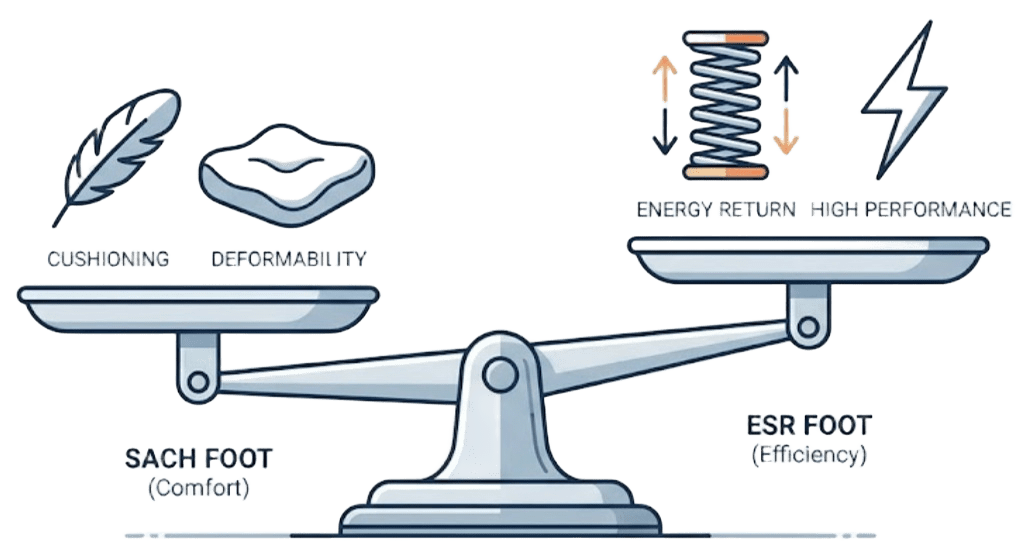
\includegraphics[width=1.0\textwidth]{image/bilancia.png}
        \end{column}
    \end{columns}
\end{frame}

\begin{frame}{Innovative Proposal: Nature's Solution}
    \begin{columns}
        % Colonna Testo (Sinistra)
        \begin{column}{0.52\textwidth}
            
            \begin{block}{The Feline Model}
                \textit{The Paw Pad} is a masterpiece of non-linear biomechanics, capable of adapting to varying impact velocities.
            \end{block}
            
            \vspace{0.2cm}
            
            \begin{block}{Anatomical Structure}
                \begin{enumerate}
                    \item \textbf{Epidermal:} Withstands intense ground interaction.
                    \item \textbf{Dermal:} Hydrostatic energy dissipation system.
                    \item \textbf{Subcutaneous:} Soft adipose tissue.
                \end{enumerate}

            \end{block}
            
            \vspace{0.2cm}
            
            \begin{alertblock}{Core Objective} % Riquadro di colore diverso (solitamente rosso/arancio)
                Translating this exact morphology into a prosthetic heel.
            \end{alertblock}
            
        \end{column}
        
        % Colonna Immagine (Destra)
        \begin{column}{0.45\textwidth}
            \hfill
            \begin{minipage}{0.9\textwidth}
                \centering
                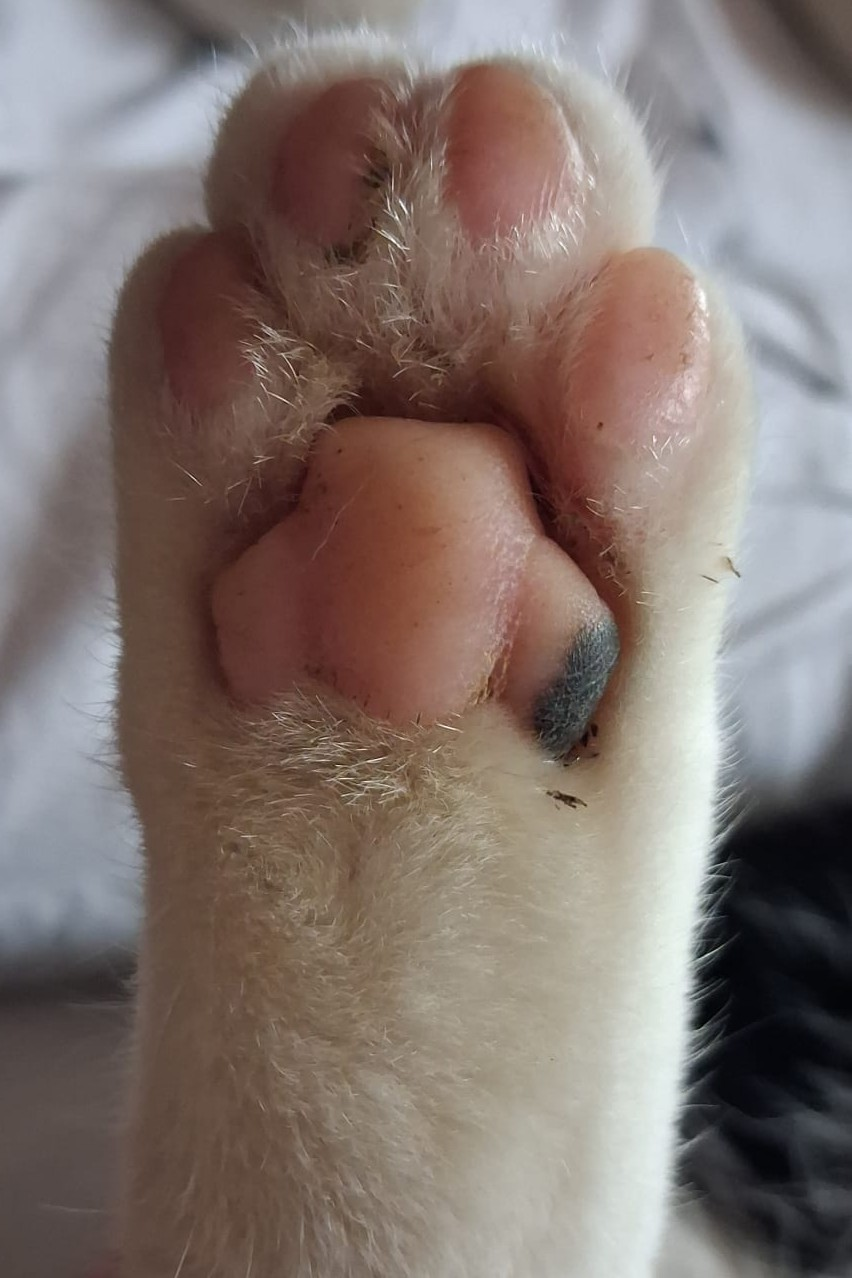
\includegraphics[width=\linewidth, height=0.45\textheight, keepaspectratio]{image/cat_pad.png}
                \vspace{0.4cm}
                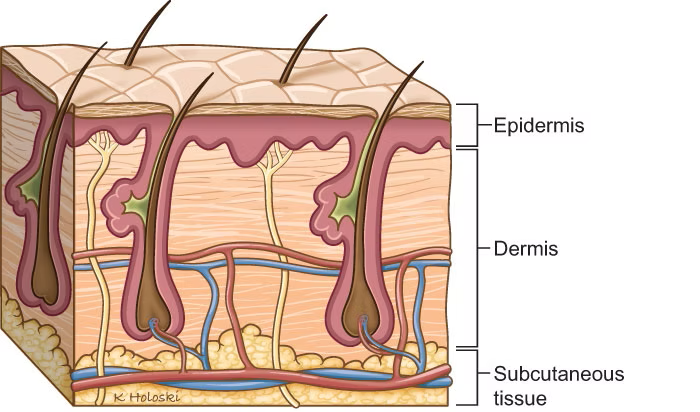
\includegraphics[width=\linewidth, height=0.35\textheight, keepaspectratio]{image/cat_layers.png}
            \end{minipage}
        \end{column}
    \end{columns}
\end{frame}

% --- INIZIO slide3_architettura_pash.tex ---
\begin{frame}{The P.A.S.H. Architecture: Engineering Paradigm Shift}
    \begin{columns}
        % Colonna Testo (Sinistra)
        \begin{column}{0.6\textwidth}
            \begin{itemize}
                \item \textbf{P.A.S.H. (Parallel Adaptive-Stiffness Heel)}
                
                \vspace{0.3cm}
                
                \item \textbf{Our Proposal: Bioinspired Parallel Architecture}
                \begin{itemize}
                    \item \textit{Elastic Component:} manages metabolic efficiency during normal gait.
                    \vspace{0.1cm}
                    \item \textit{Bio-inspired Damper (STF):} "activates" only to absorb extreme impacts, without interfering at low speeds.
                \end{itemize}
                
                \vspace{0.3cm}
                
                \item \textbf{Result:} perfect synergy between mechanical design and \textit{Smart Materials}.
            \end{itemize}
        \end{column}
        
        % Colonna Immagine (Destra)
        \begin{column}{0.45\textwidth}
            \centering
            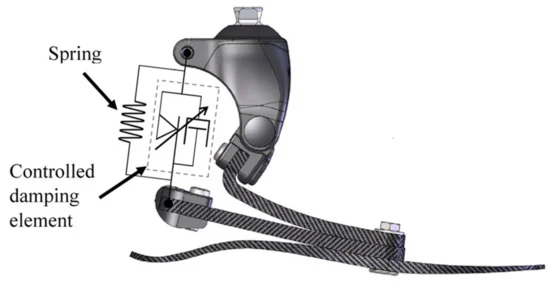
\includegraphics[width=0.85\textwidth]{image/parallel_architecture.png}
        \end{column}
    \end{columns}
\end{frame}


% --- SLIDE 7: CONCEPT DEVELOPMENT (STRUTTURA) ---
\begin{frame}{Concept Development: Components and Materials}
    
    \vspace{0.4cm}
    
    % Le tre colonne allineate in alto (opzione [T])
    \begin{columns}[T]
        
        % --- 1. ELASTIC COMPONENT ---
        \begin{column}{0.31\textwidth}
            \centering
            % INSERISCI QUI LA TUA PRIMA FOTO
            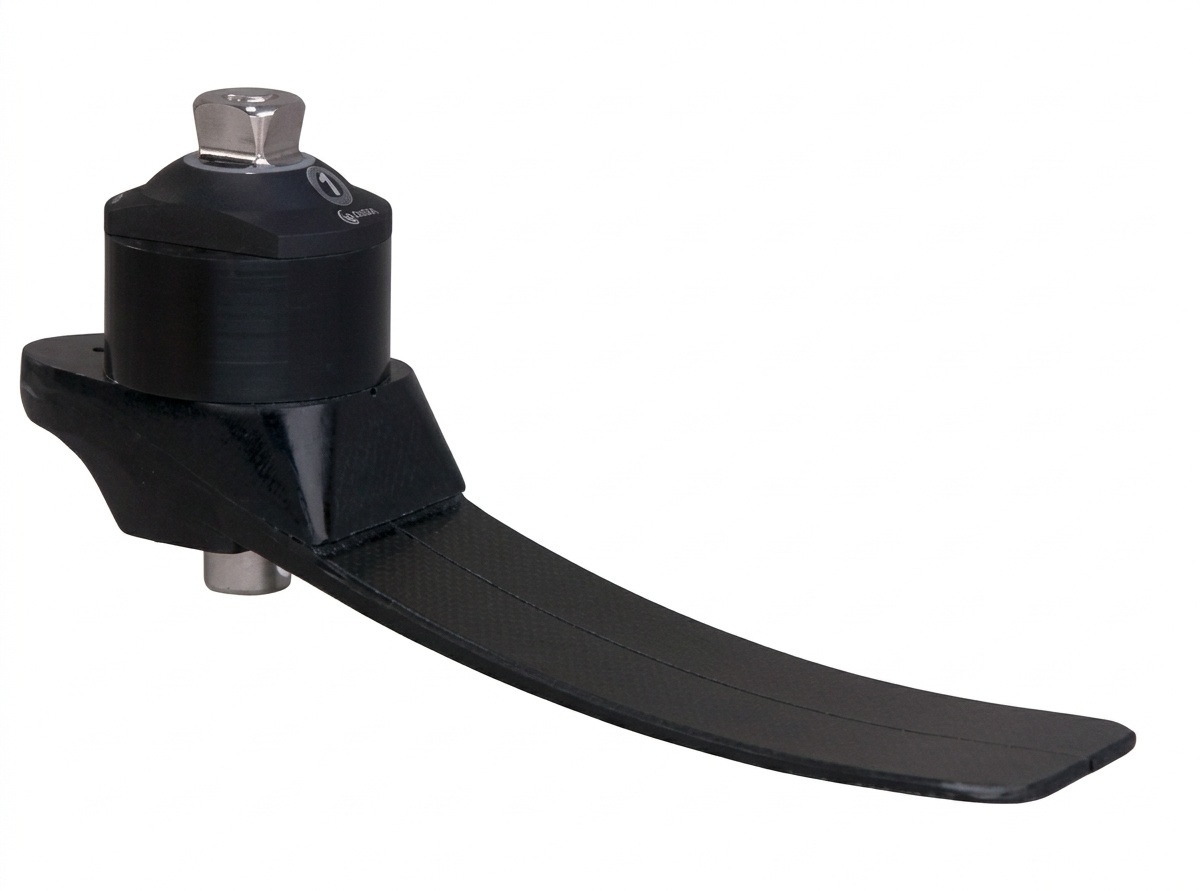
\includegraphics[width=0.95\linewidth]{image/foto_lamina.png} 
            
            \vspace{0.3cm}
            \begin{block}{1. Elastic Component}
                \scriptsize \textbf{ESR Carbon Fiber Blade:} Acts as the main tendon. Manages the \textit{Toe-off} phase and stores propulsive energy.
            \end{block}
        \end{column}
        
        % --- 2. STRUCTURAL MATRIX ---
        \begin{column}{0.34\textwidth}
            \centering
            % INSERISCI QUI LA TUA SECONDA FOTO
            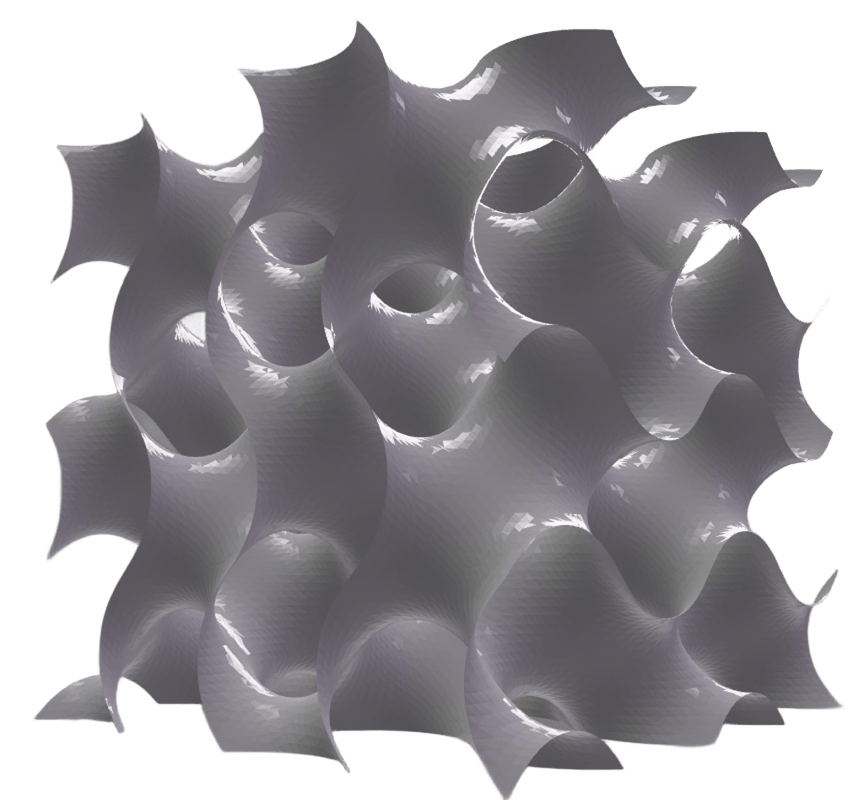
\includegraphics[width=0.87\linewidth]{image/Gyroid.png} 
            
            \vspace{0.08cm}
            \begin{block}{2. Structural Matrix}
                \scriptsize \textbf{Dermal Layer (TPMS):} Flexible TPU scaffold with gyroid structure. Sustains the baseline load and guides the spatial deformation.
            \end{block}
        \end{column}
        
        % --- 3. INTELLIGENT CORE ---
        \begin{column}{0.31\textwidth}
            \centering
            % INSERISCI QUI LA TUA TERZA FOTO
            \vspace{0.45cm}
            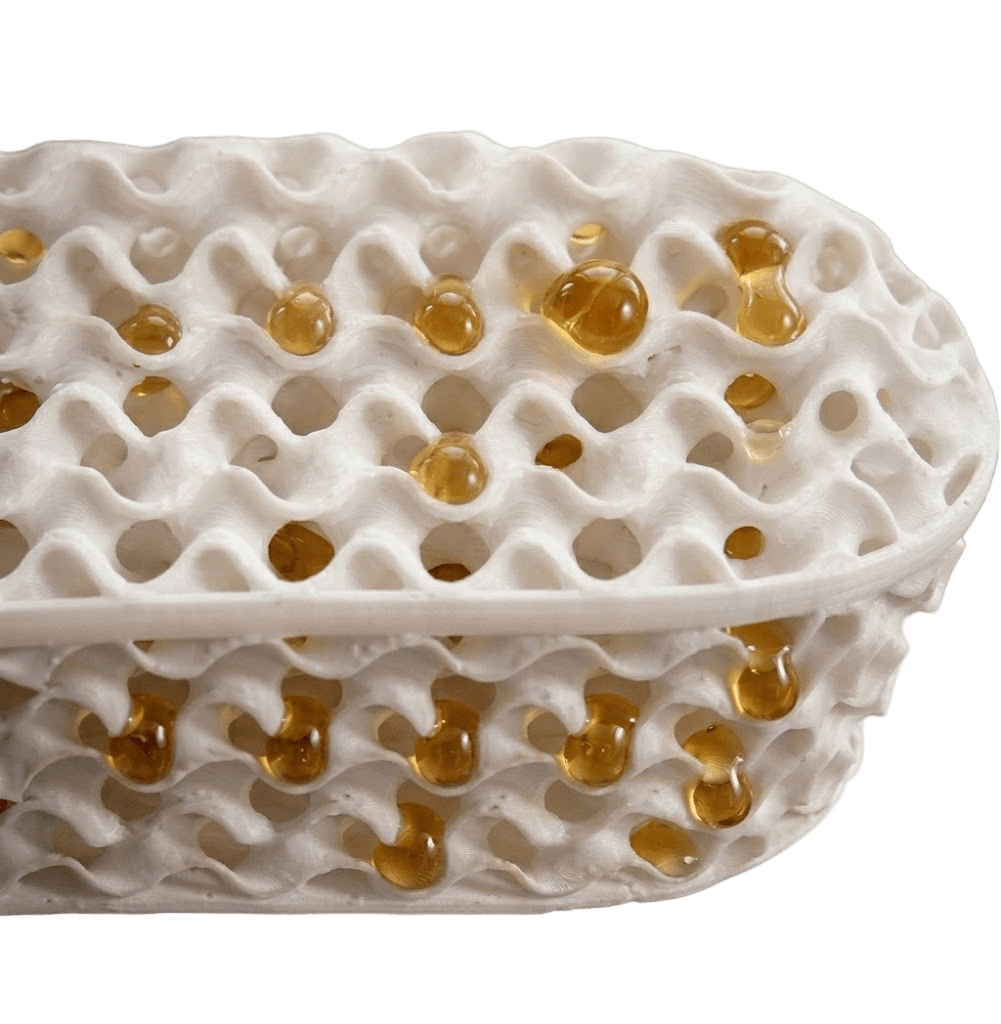
\includegraphics[width=0.95\linewidth]{image/foto_stf.png} 
            
            \vspace{-0.35cm}
            \begin{block}{3. Intelligent Core}
                \scriptsize \textbf{Adipose Tissue (STF):} Confined non-Newtonian fluid (suspension of $SiO_2$ nanoparticles in PEG). Modulates stiffness based on impact velocity.
            \end{block}
        \end{column}
        
    \end{columns}
\end{frame} % Sardo

% --- SLIDE 8: CONCEPT DEVELOPMENT (DINAMICA) ---
\begin{frame}{Concept Development: Smart Dynamic Response of STF}

    \vspace{-0.3cm}
    % --- NUOVA SEZIONE CON IMMAGINE CENTRATA ---
    % Sostituisci 'percorso_della_tua_immagine' con il file reale
    % Puoi regolare width o scale per ottimizzare la dimensione
    \begin{center}
        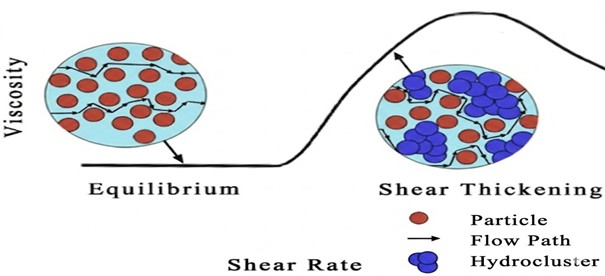
\includegraphics[width=0.45\textwidth,keepaspectratio]{image/graficoSTF.jpg}
    \end{center}
    % ---------------------------------------------

    \vspace{-0.45cm} % Spazio verticale ridotto leggermente per bilanciare con l'immagine

    \begin{columns}[T]
        % Box Sinistra: Camminata
        \begin{column}{0.48\textwidth}
            \begin{alertblock}{Low Shear Rate (Walk, $Fr < 0.5$)}
                \begin{itemize}
                    \item \textbf{STF State:} Low viscosity (Fluid).
                    \item \textbf{Mechanics:} The TPMS matrix deforms elastically under the load.
                    \item \textbf{Cushioning:} The heel "sinks" to absorb terrain irregularities.
                    \item \textbf{Result:} Natural \textit{roll-over}, optimal damping without triggering the stiff blade.
                \end{itemize}
            \end{alertblock}
        \end{column}

        % Box Destra: Corsa
        \begin{column}{0.48\textwidth}
            \begin{exampleblock}{High Shear Rate (Run, $Fr > 0.5$)}
                \begin{itemize}
                    \item \textbf{STF State:} Instant solidification.
                    \item \textbf{Mechanics:} The damper locks its volumetric deformation.
                    \item \textbf{Bridging:} The heel becomes a rigid bridge, dissipating zero energy.
                    \item \textbf{Result:} Ground Reaction Forces (GRF) are fully transferred to the blade for propulsion.
                \end{itemize}
            \end{exampleblock}
        \end{column}
    \end{columns}
\end{frame} % Sardo

% --- SLIDE 9: TECHNICAL FEASIBILITY (SINGLE SLIDE) ---
\begin{frame}{Technical Feasibility}
    % Layout pulito con elenchi puntati per massima leggibilità
    \begin{columns}[T]
        \begin{column}{0.95\textwidth}
            \small
            \begin{itemize}
                \item \textbf{1. Kinematic Response (The "Wall Effect" Risk)}
                \begin{itemize}
                    \item \textit{Challenge:} Preventing premature STF hardening during oblique heel strikes at low speeds.
                    \item \textit{Solution:} \alert{Rheological Tuning}. By precisely adjusting the $SiO_2$ mass fraction, we calibrate the \textit{critical shear rate} to ensure activation occurs only during high-energy tasks.
                \end{itemize}
                
                \vspace{0.4cm}
                
                \item \textbf{2. Pendulum Effect (Distal Inertia)}
                \begin{itemize}
                    \item \textit{Challenge:} Fluid mass increases the distal weight, raising metabolic cost during the \textit{Swing Phase}.
                    \item \textit{Solution:} \alert{Spatial Optimization}. STF is not distributed uniformly but encapsulated strictly within primary load-bearing lobes, reducing fluid weight by $\sim$60\% without performance loss.
                \end{itemize}
                
                \vspace{0.4cm}
                
                \item \textbf{3. Material Fatigue \& Leakage}
                \begin{itemize}
                    \item \textit{Challenge:} Cyclic loading ($10^6$ cycles) leading to TPU micro-fractures and fluid leakage.
                    \item \textit{Solution:} \alert{Micro-compartmentalization}. The closed-cell TPMS structure ensures a \textit{fail-safe} design. A localized puncture results in negligible performance degradation instead of catastrophic failure.
                \end{itemize}
            \end{itemize}
        \end{column}
    \end{columns}
\end{frame} % Sardo

\begin{frame}{Cost Analysis \& Production }
   
    % BLOCCO 1: INPUT (Materiali)
    \begin{tcolorbox}[enhanced, title=\textbf{1. Bill of Materials (Unit Cost)}, 
        colframe=blue!80!black, colback=blue!5, 
        boxrule=0.5mm, arc=1.5mm, drop fuzzy shadow]
        \begin{itemize}
            \item \textbf{ESR Carbon Fiber:} $\sim$100 \texteuro  \hspace{0.05cm}
                  \textbf{TPU Scaffold:} $\sim$10 \texteuro \hspace{0.05cm}
                  \textbf{STF Matrix (PEG + $SiO_2$):} $<5$ \texteuro
        \end{itemize}
    \end{tcolorbox}
    


    % BLOCCO 2: PROCESSO (Produzione)
    \begin{tcolorbox}[enhanced, title=\textbf{2. Production \& Assembly}, 
        colframe=gray!80!black, colback=gray!5, 
        boxrule=0.5mm, arc=1.5mm, drop fuzzy shadow]
        %\vspace{-0.1cm}
        \begin{itemize}
            \item \textbf{Prototyping:} SLS 3D Printing (TPU) + Nesting optimization.
            \item \textbf{Assembly:} Rapid mechanical sealing ($<$1h), highly standardized.
        \end{itemize}
    \end{tcolorbox}
    

    % BLOCCO 3: OUTPUT (Vantaggio Competitivo)
    \begin{tcolorbox}[enhanced, title=\textbf{3. Market Disruption}, 
        colframe=red!70!black, colback=red!5, 
        boxrule=0.5mm, arc=1.5mm, drop fuzzy shadow]
        %\vspace{-0.1cm}
        \begin{itemize}
            \item \textbf{Zero Electronics:} No CapEx for sensors, batteries, or microcontrollers.
            \item \textbf{Low TCO (Total Cost of Ownership):} Passive design eliminates software calibration.
            \item \textbf{Target Cost:} $\sim$500 \texteuro \ (P.A.S.H.) vs $>5000$ \texteuro \ (Active Bionic Alternatives).
        \end{itemize}
    \end{tcolorbox}

\end{frame}
% --- SLIDE 10: USE CASES ---
\begin{frame}{Applications \& Use Cases}

    \begin{columns}[T]

        % ── Colonna SINISTRA ──
        \begin{column}{0.32\textwidth}

            \setbeamercolor{block body}{bg=colorWalking, fg=blockText}
            \setbeamercolor{block title}{bg=colorWalking!80!black, fg=white}
            \begin{block}{\small Prosthetic Feet}
                \footnotesize \textit{(Transtibial / Transmetatarsal)}\\[0.2em]
                Passive stiffness tuning across all prosthesis levels — from partial foot to transtibial. \textbf{No electronics}, no recalibration required.
            \end{block}

            \vspace{\fill}
            \vspace{0.15cm}

            \setbeamercolor{block body}{bg=colorTerrain, fg=blockText}
            \setbeamercolor{block title}{bg=colorTerrain!80!black, fg=white}
            \begin{block}{\small Smart Insoles}
                \footnotesize \textit{(Runners / Astronauts)}\\[0.2em]
                Adaptive heel cushioning for \textbf{intact limbs}: terrain-blind impact absorption in high-load or \textit{microgravity} re-adaptation contexts.
            \end{block}

        \end{column}
        
        % ── Colonna CENTRALE (foto) ──
        \begin{column}{0.34\textwidth}
            \vspace{0.3cm}
            \begin{center}
                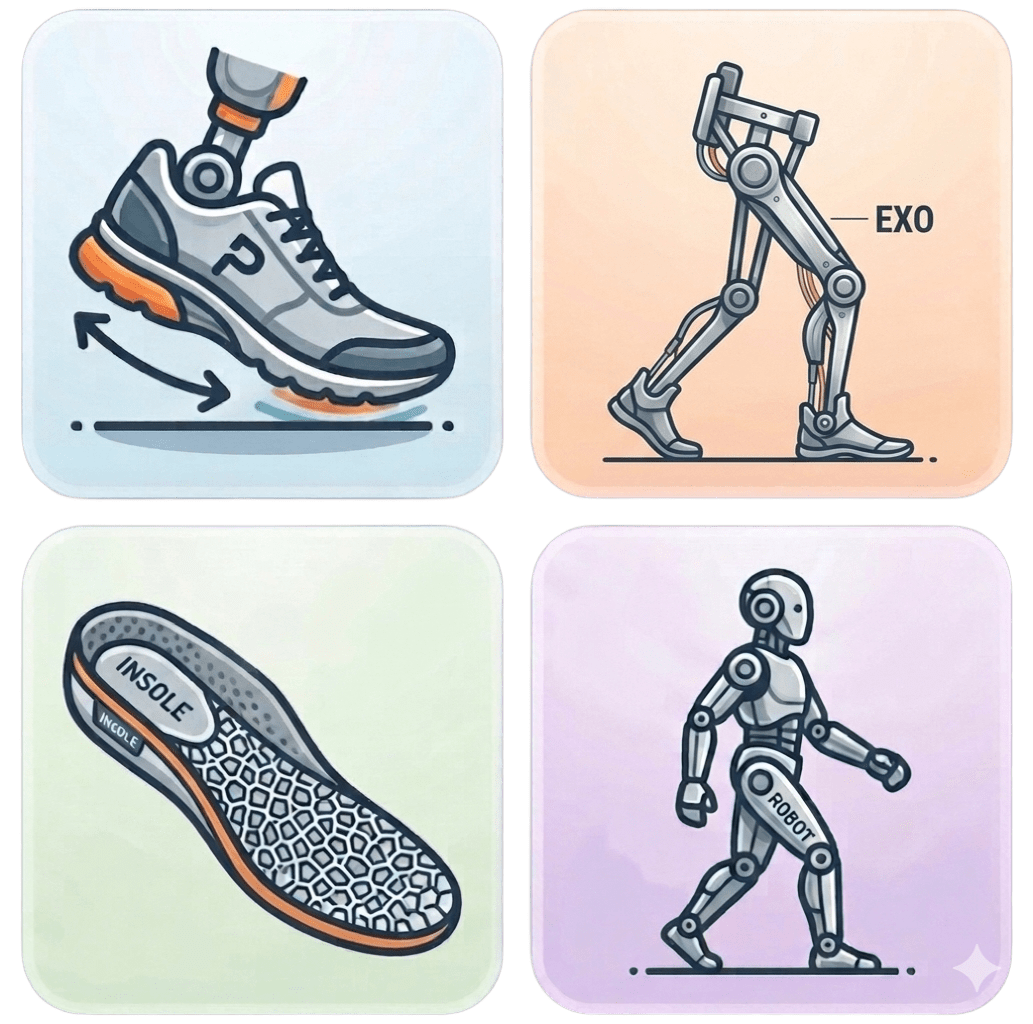
\includegraphics[width=\linewidth, height=4.8cm, keepaspectratio]{image/usecases.png}
            \end{center}
        \end{column}

        % ── Colonna DESTRA ──
        \begin{column}{0.32\textwidth}

            \setbeamercolor{block body}{bg=colorRunning, fg=blockText}
            \setbeamercolor{block title}{bg=colorRunning!80!black, fg=white}
            \begin{block}{\small Exoskeletons}
                \footnotesize \textit{(Rehabilitation / Industrial)}\\[0.2em]
                Compliant heel module for lower-limb exoskeletons: impact attenuation at \textbf{Heel Strike} without added actuators or control loops.
            \end{block}

            \vspace{0.15cm}

            \setbeamercolor{block body}{bg=colorAccess, fg=blockText}
            \setbeamercolor{block title}{bg=colorAccess!80!black, fg=white}
            \begin{block}{\small Bipedal Robots}
                \footnotesize \textit{(Humanoid / Legged Systems)}\\[0.2em]
                Passive heel compliance reduces \textbf{Ground Reaction Force} peaks at Heel Strike — no sensors, no control overhead.
            \end{block}

        \end{column}

    \end{columns}

    \vspace{0.15cm}
    \centering

\end{frame}
\begin{frame}{FelixStride: \textit{The next step in passive prostethics}}
    \vspace{-0.3cm}

    \begin{columns}[T]
        % COLONNA SINISTRA: ROADMAP E FONDI
        \begin{column}{0.62\textwidth}
            \
            % ZONA 1: TRL 1-3
            \begin{tcolorbox}[enhanced, title=\small \textbf{Phase 1: Proof of Concept (TRL 1-3)}, 
                colframe=blue!70!black, colback=blue!5, boxrule=0.3mm, arc=1mm]
                \footnotesize
                \textbf{Focus:} Lab validation \& STF/TPU optimization.\\
                \textbf{Funding:} MIMIT PoC Grants, Regional FESR (Azione 1.3.1).
            \end{tcolorbox}

           
            \vspace{0.3cm}
            % ZONA 2: TRL 4-6 (VALLEY OF DEATH)
            \begin{tcolorbox}[enhanced, title=\small \textbf{Phase 2: The Critical Gap (TRL 4-6)}, 
                colframe=red!70!black, colback=red!5, boxrule=0.5mm, arc=1mm]
                \footnotesize
                \textbf{Focus:} Prototype scaling \& Pilot clinical studies.\\
                \textbf{Funding:} Seed VC, STEP (Strategic Tech for Europe), SME Funds.
            \end{tcolorbox}

            \vspace{0.3cm}

            % ZONA 3: TRL 7-9
            \begin{tcolorbox}[enhanced, title=\small \textbf{Phase 3: Market Entry (TRL 7-9)}, 
                colframe=green!60!black, colback=green!5, boxrule=0.3mm, arc=1mm]
                \footnotesize
                \textbf{Focus:} MDR Compliance (CE), Full Clinical Trials, Global Launch.\\
                \textbf{Funding:} EIC Accelerator, MIMIT Biomedical Fund, EIT Health.
            \end{tcolorbox}
        \end{column}
       
        % COLONNA DESTRA: LOGO E GRAFICO
        \begin{column}{0.35\textwidth}
            \begin{center}
                \vspace{-0.3cm}
                 
\includegraphics[height=3cm]{image/FelixStride_logo.png}
                
              
                
                \begin{tcolorbox}[enhanced, colframe=red!70!black, colback=white, boxrule=0.4mm, 
                    title=\tiny \textbf{FINANCIAL CHALLENGE}]
                    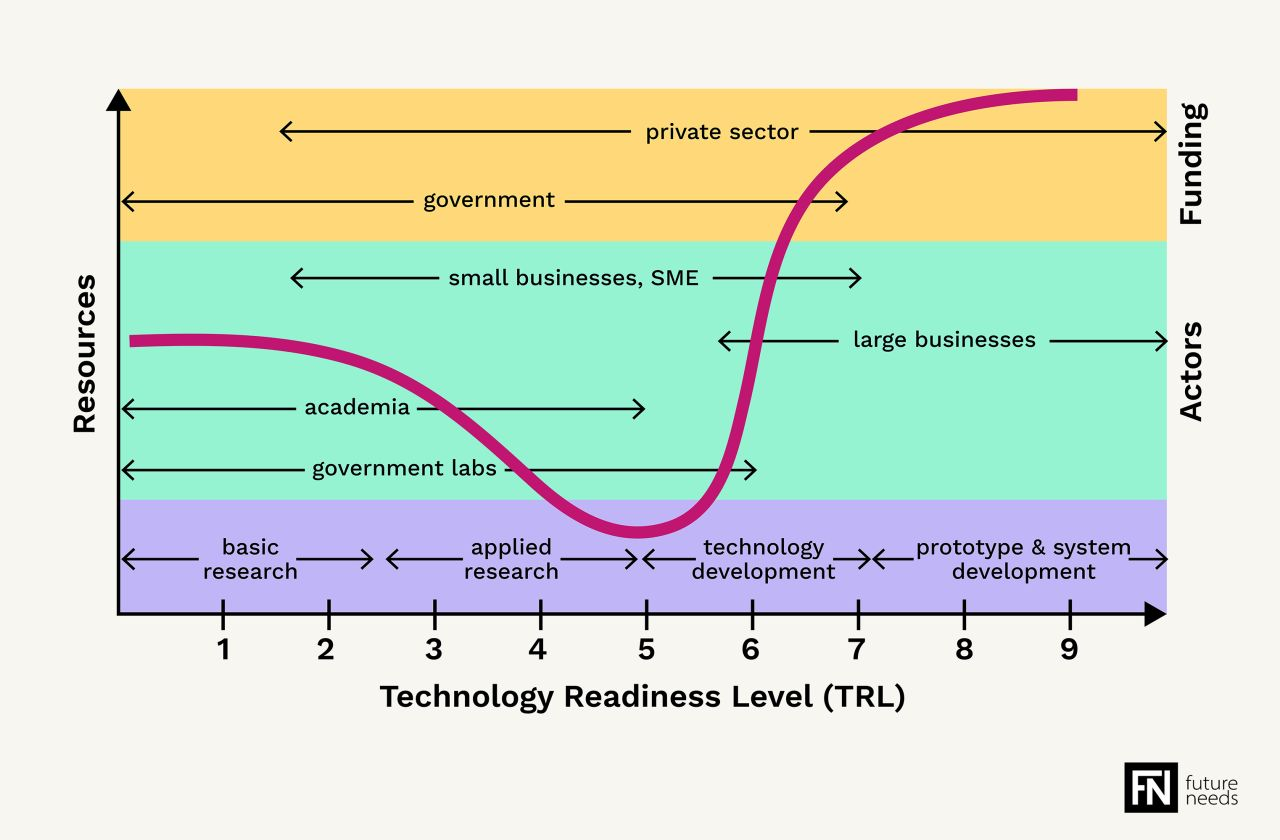
\includegraphics[width=\textwidth]{image/Valley_ofDeath.jpeg}
                    \vspace{0.1cm}
                    \centering \tiny \textit{Bridging TRL 4 to 7 via Seed \& STEP Grants.}
                \end{tcolorbox}
            \end{center}
        \end{column}
    \end{columns}
\end{frame} % Ric

\begin{frame}{References \& Further Reading}
    \begin{columns}
        \begin{column}{0.6\textwidth}
            \footnotesize
            \begin{itemize}
                \item \textbf{ Y. Xiao et al.}, \textit{"A 3D-Printed Sole Design Bioinspired by Cat Paw Pad..."}, Polymers, vol. 14, no. 16, p. 3270, 2022.
                \vspace{0.3cm}
                \item \textbf{ H. Tryggvason et al.}, \textit{"Use of Dynamic FEA for Design Modification and Energy Analysis of a Variable Stiffness Prosthetic Foot,"} Applied Sciences, vol. 10, no. 2, p. 650, 2020.
                \vspace{0.3cm}
                \item \textbf{Energy Dissipation:} \\ Smith \& Doe (2019), \textit{Nat. Biomech.}
            \end{itemize}
        \end{column}
        
        \begin{column}{0.4\textwidth}
            \centering
            \textbf{Full Bibliography}\\
            \vspace{0.3cm}
            % Sostituisci "example-image" con il file del tuo QR code
            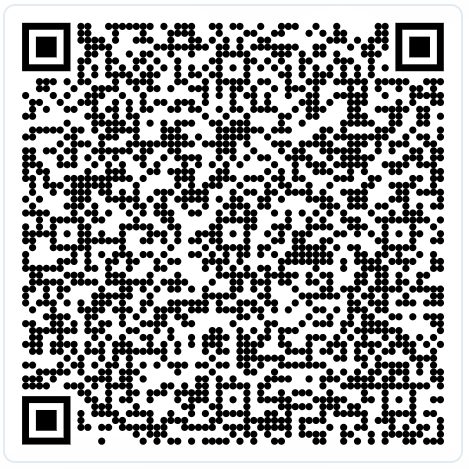
\includegraphics[width=0.7\linewidth]{image/Qr_COde.png}
            \vspace{0.2cm}
            \\
            \begin{tiny}
                \texttt{Scan to access the full literature database}
            \end{tiny}
        \end{column}
    \end{columns}
\end{frame}
\end{document}